\section{hlavná stránka}
\subsection{hlavná stránka}
\label{hlavná stránka}
\begin{frame}\frametitle{hlavná stránka}
  \begin{figure}[htb]
    \centering
    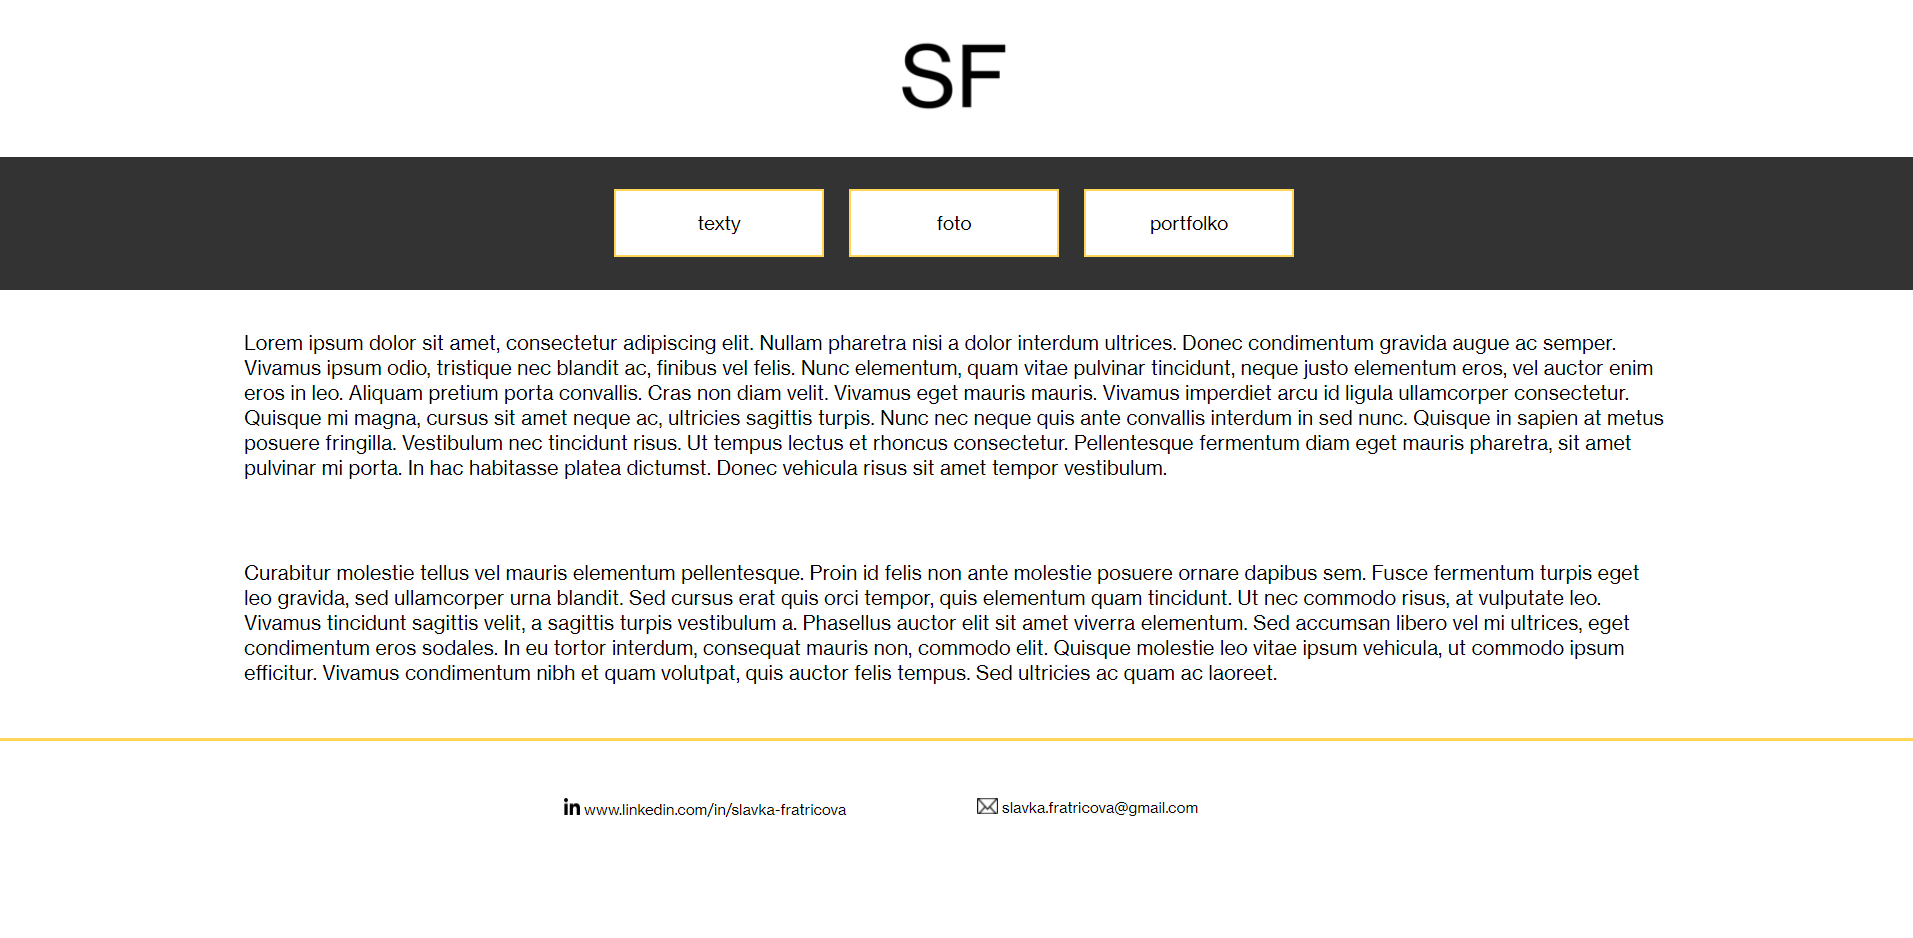
\includegraphics[scale=0.3]{uvodka.png}
    \caption{hlavná stránka}
  \end{figure}

\end{frame}

\subsection{texty}
\begin{frame}\frametitle{texty}
  \begin{figure}[htb]
    \centering
    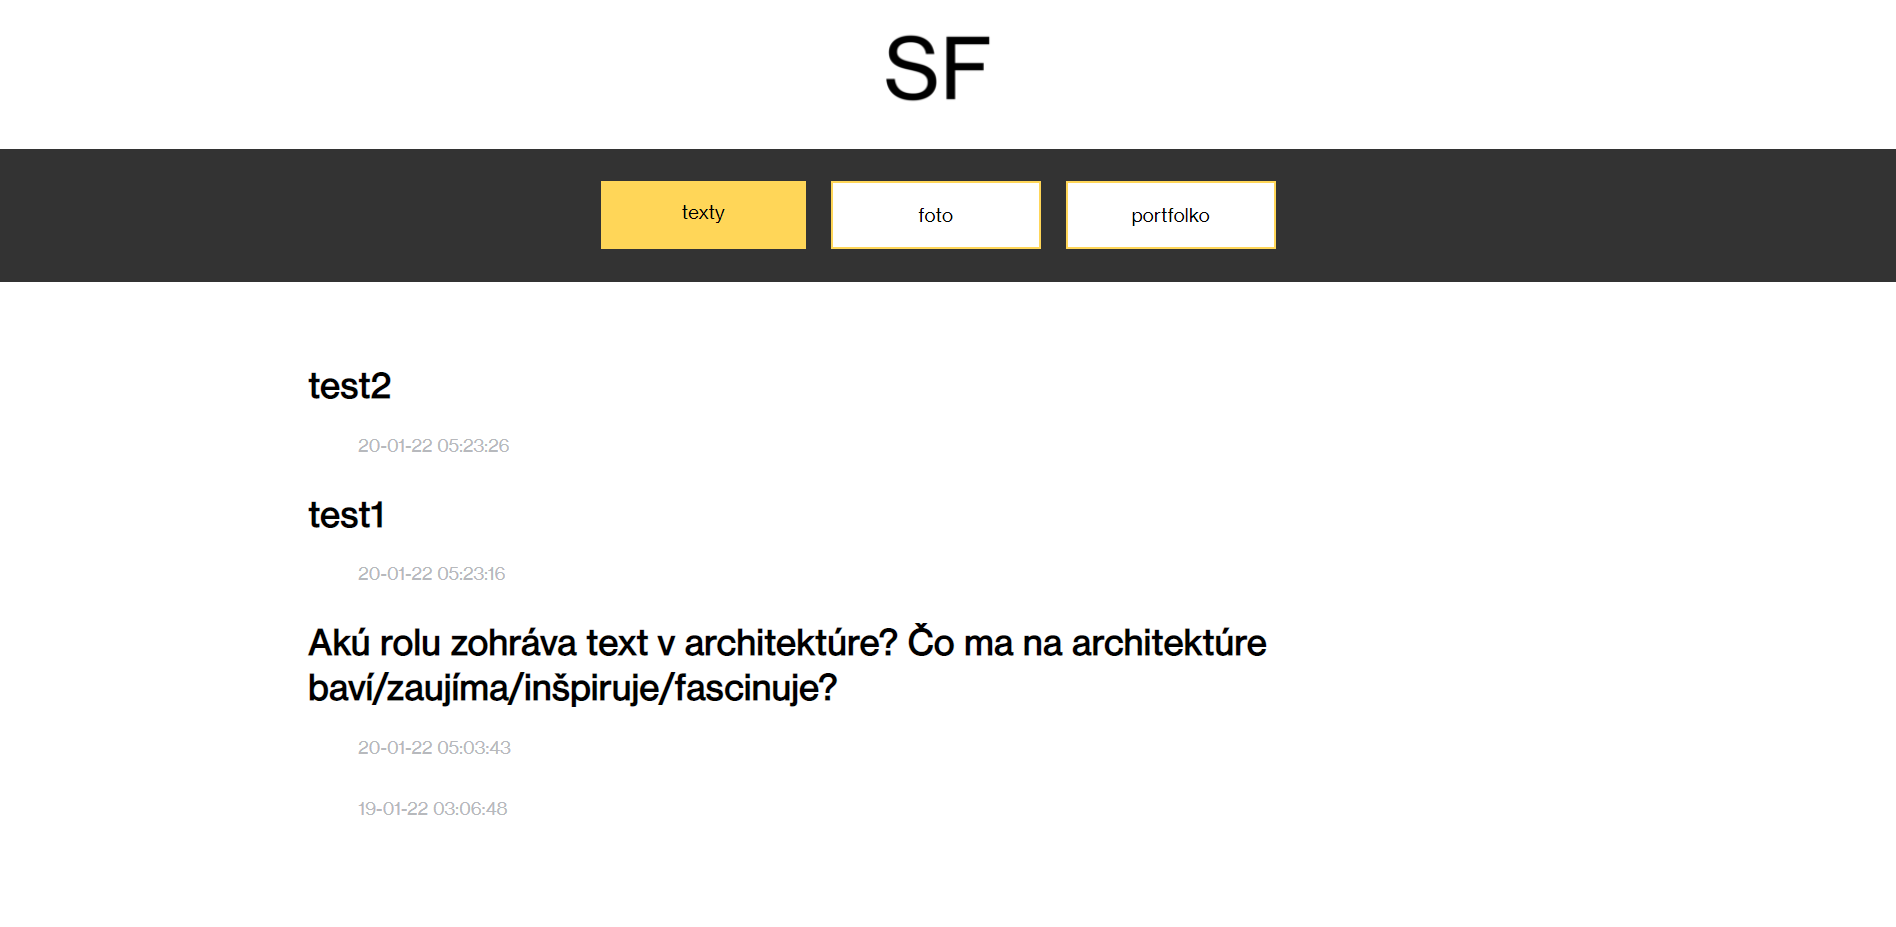
\includegraphics[scale=0.3]{texty_bez_text.png}
    \caption{texty}
  \end{figure}

\end{frame}

\subsection{fotografie}
\begin{frame}\frametitle{fotografie}
  \begin{figure}[htb]
    \centering
    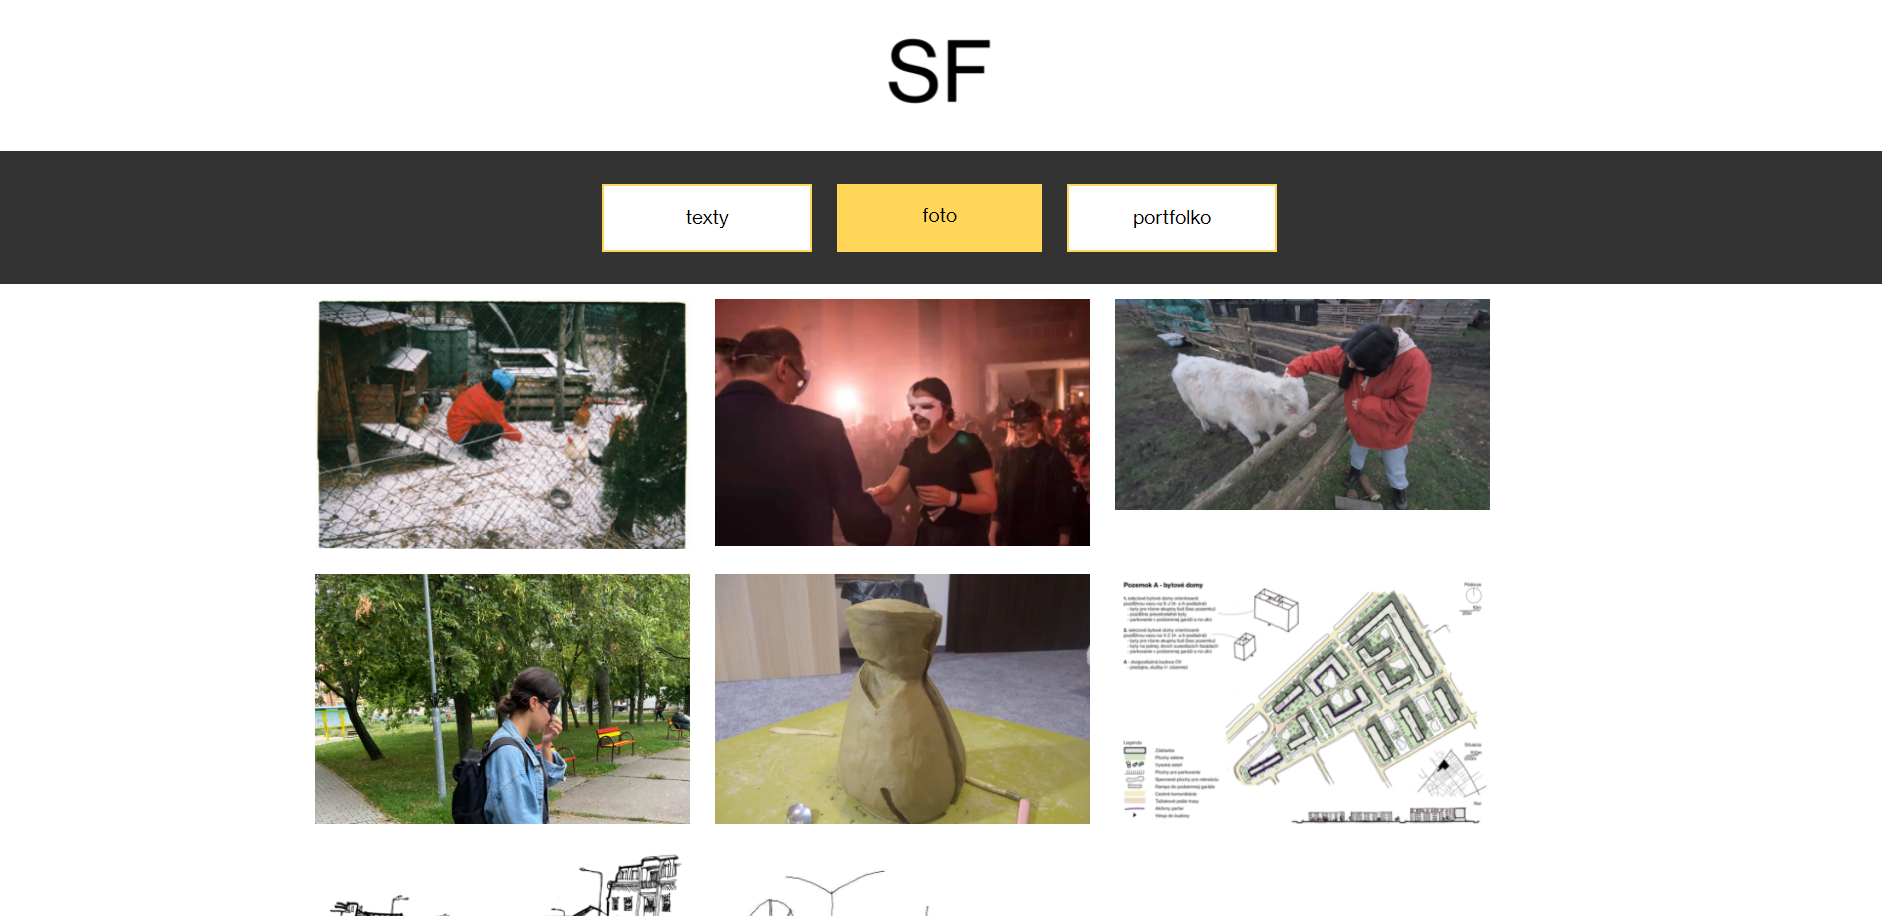
\includegraphics[scale=0.3]{galeria.png}
    \caption{fotografie}
  \end{figure}

\end{frame}

\subsection{portfólio}
\begin{frame}\frametitle{portfólio}
  \begin{figure}[htb]
    \centering
    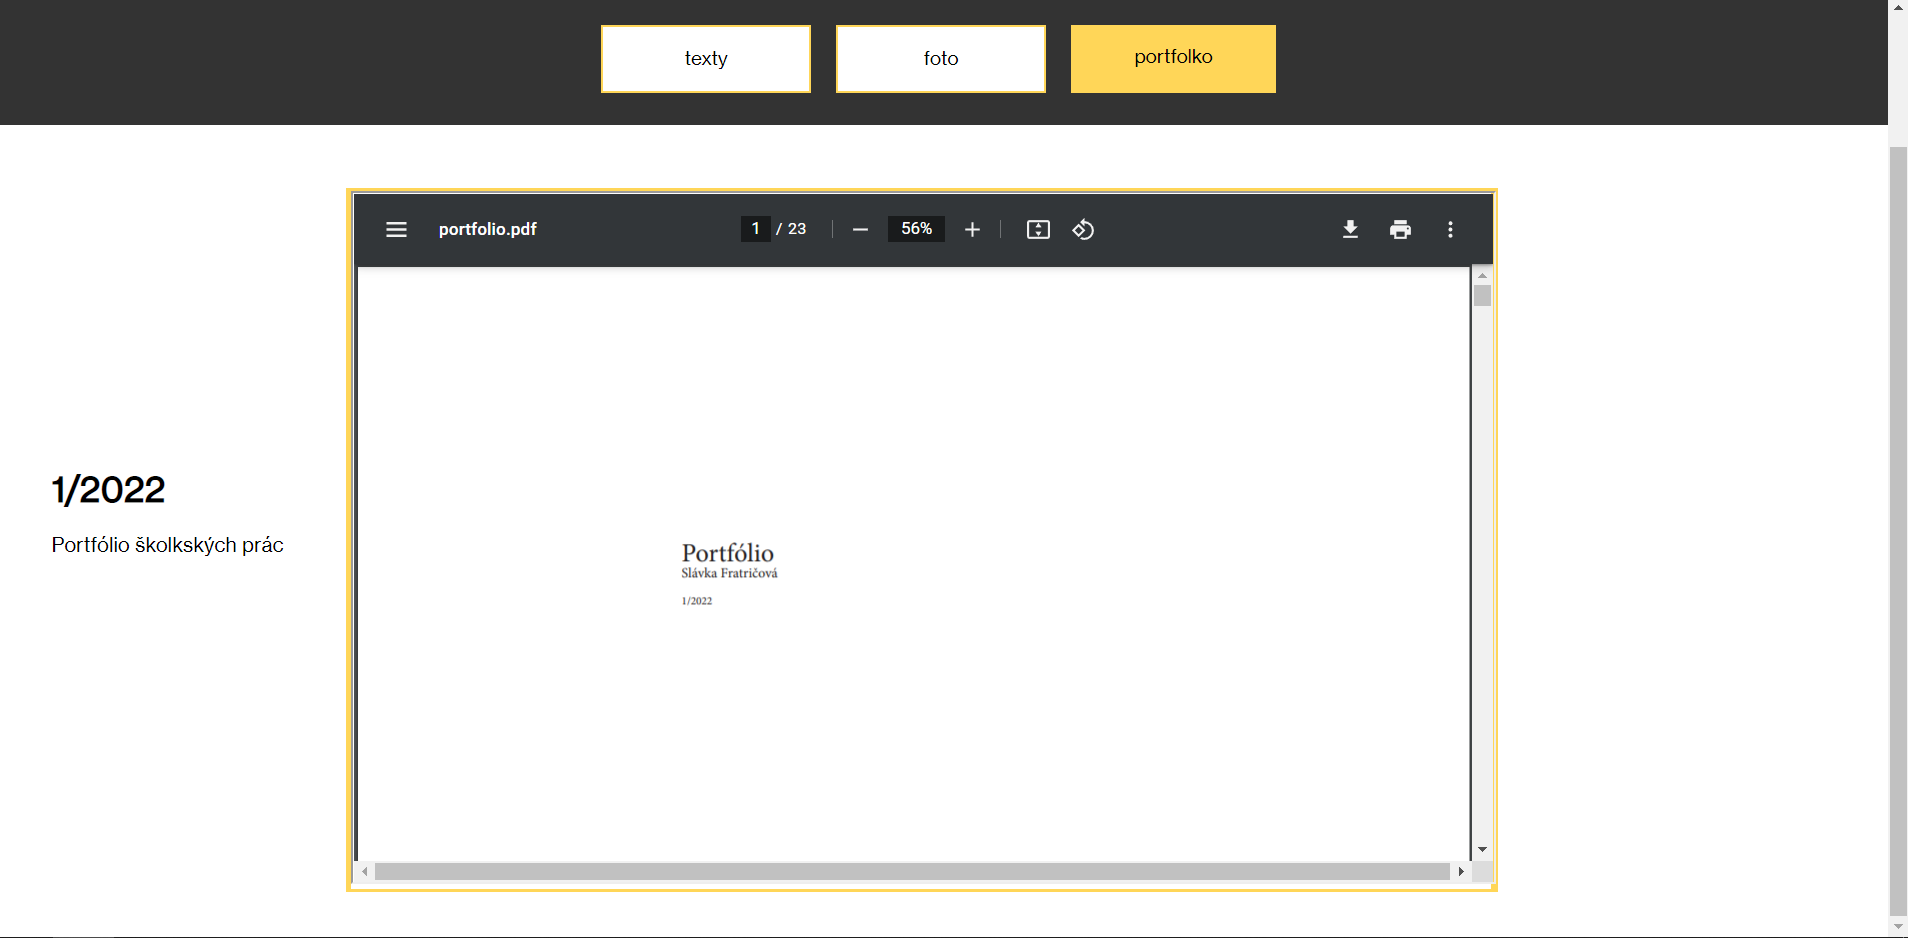
\includegraphics[scale=0.3]{portfolko.png}
    \caption{portfólio}
  \end{figure}

\end{frame}
\section{Administrátorské prostredie}
\subsection{Administrátorské prostredie}

\begin{frame}\frametitle{Administrátorské prostredie}
Stránka bola tvorená pre klienta bez znalostí programovania v prostredí php
a MySQL, tým pádom musí byť nastavovanie všetkých parametrov stránok veľmi intuitívne a najlepšie tvorené pomocou formulárov s nápismi čo treba robiť a kam pridať aké
formáty súborov. Z toho dôvodu je vytvorené programátorské prostredie, ktoré je ale zabezpečené pred nechceným vstupom menom a heslom.

 \begin{itemize}
 \item Funkcie admin:
           \begin{itemize}
          \item upload image: pridávanie fotiek do podstránky foto.php
          \item add post: pridávanie článkov do podstránky indexx.php
          \item manage post: úprava článkov podstránky indexx.php
          \item reset your password: reset hesla
          \item sign out of your account: odhlásiť sa z prostredia admin.php
          \item register new account: registrácia nového admina
          \item home: presmerovanie na index.php
         \end{itemize}
 \end{itemize}


\end{frame}

\begin{frame}\frametitle{Administrátorské prostredie}
  \begin{figure}[htb]
    \centering
    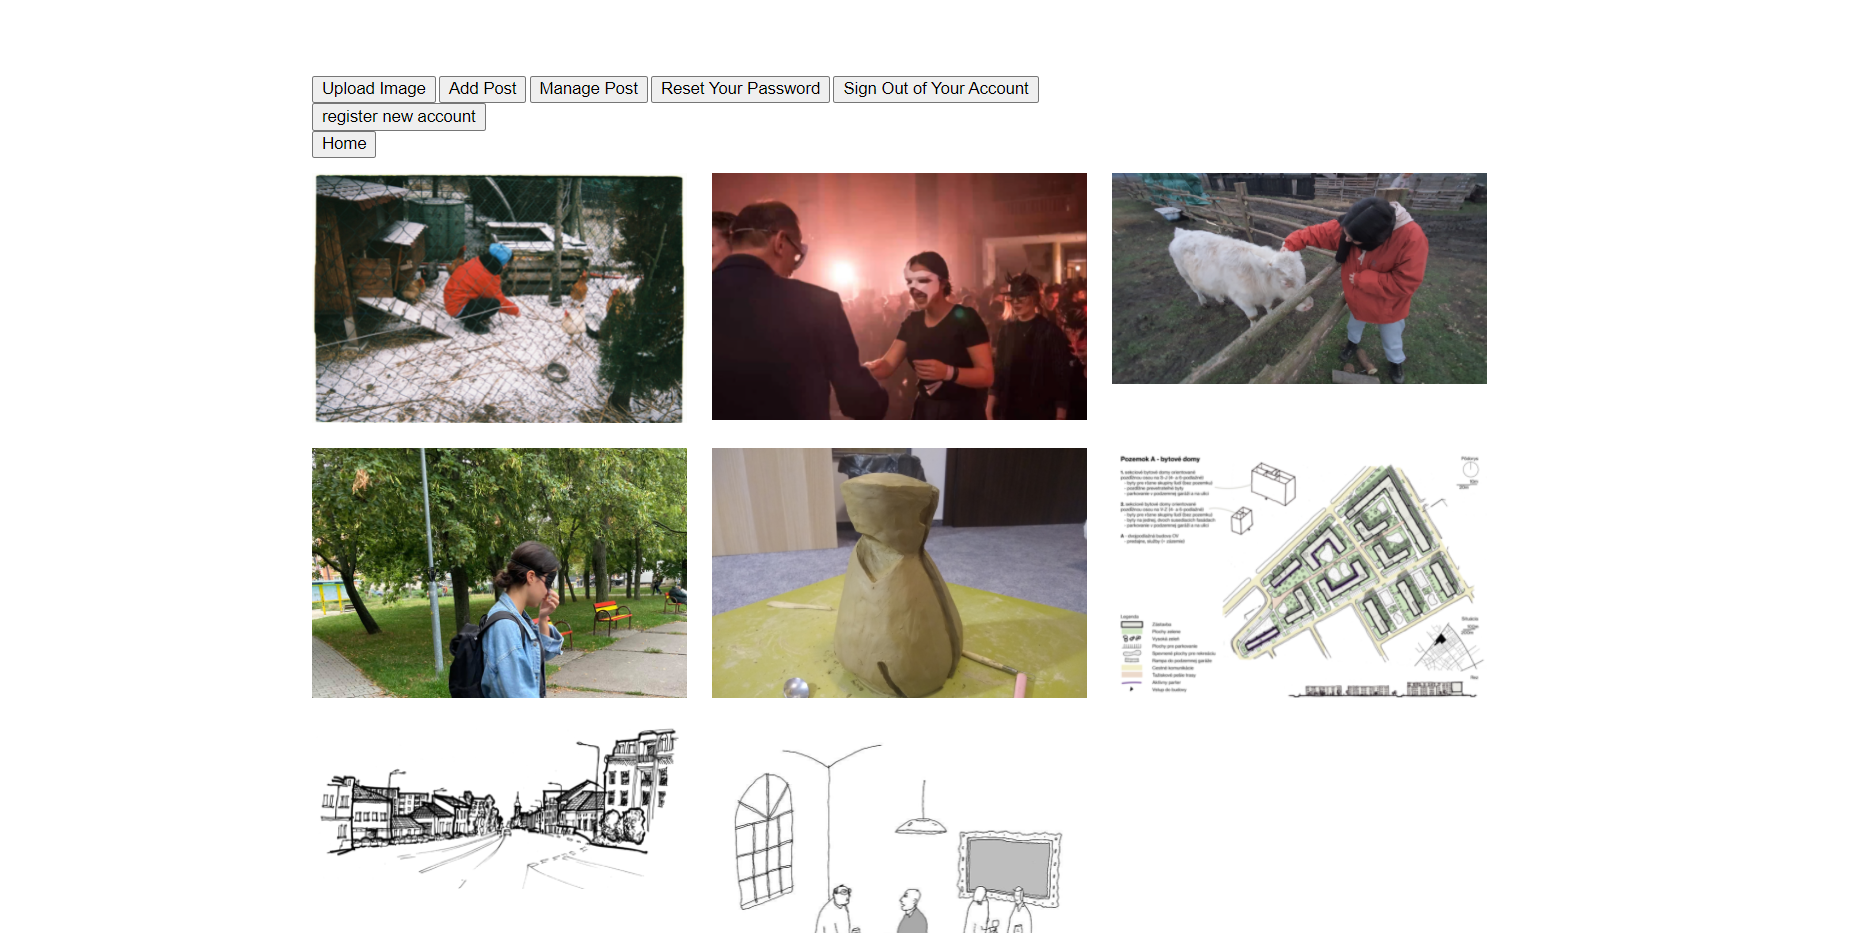
\includegraphics[scale=0.30]{admin.png}
    \caption{Administrátorské prostredie}
  \end{figure}
\end{frame}
